The CLAS detector has two major subsystems, the central detector and the forward detectors, as well as a forward tagger and backward angle neutron detector (BAND)

    \begin{figure}[H]
        \centering
        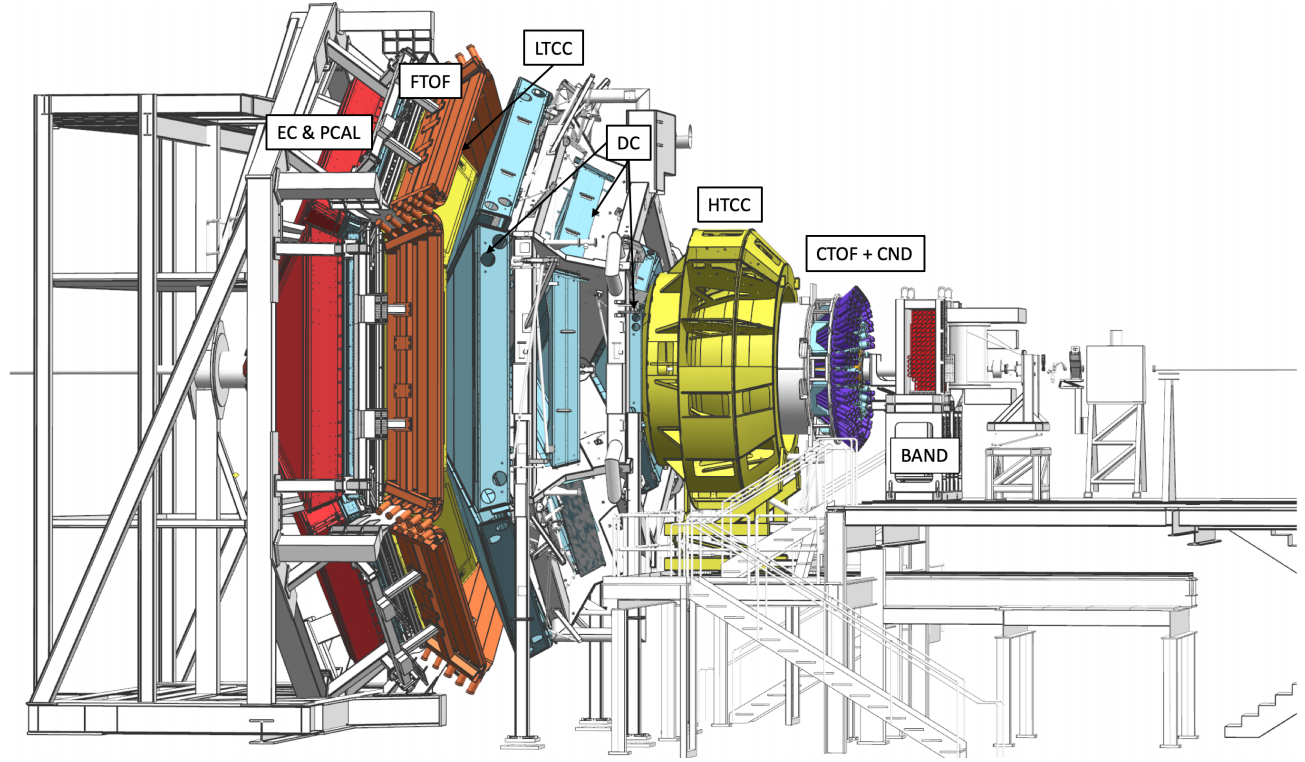
\includegraphics[width=12cm]{Chapters/Ch2-Experiment/clas-12-exp/clas-detectors/other/pics/CLAS12.png}
        \caption{ CLAS12 Detector System }
    \end{figure}
    
    \begin{figure}[H]
        \centering
        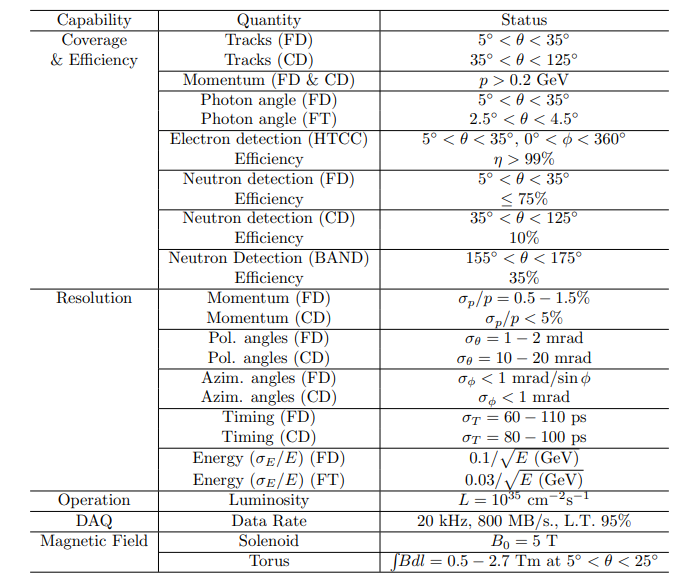
\includegraphics[width=10cm]{Chapters/Ch2-Experiment/clas-12-exp/clas-detectors/other/pics/clas12-params.png}
        \caption{CLAS12 Specification}
    \end{figure}

    \begin{figure}[H]
        \centering
        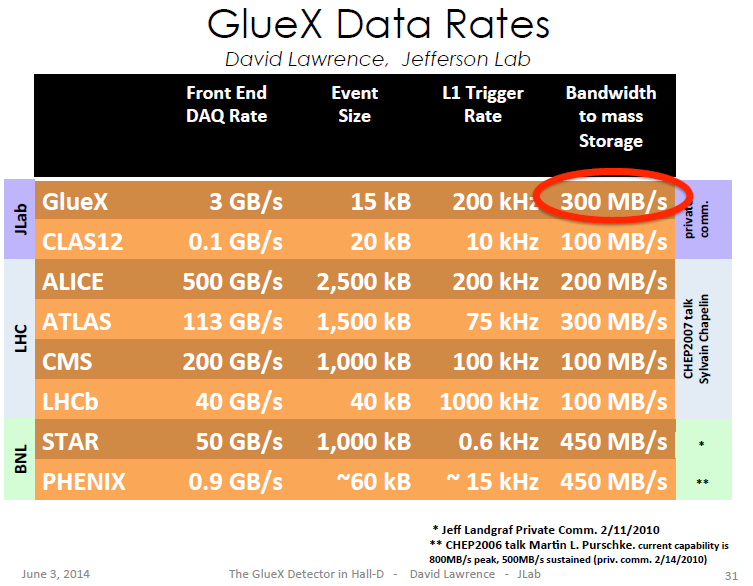
\includegraphics[width=10cm]{Chapters/Ch2-Experiment/clas-12-exp/clas-detectors/other/pics/good_data_rates_slide.png}
        \caption{CLAS12 Data Rates, Compared to Other Experiments }
    \end{figure}

    \todo{include note about HofstaderM. Gockeler et al., Phys.Rev.Lett. 98, 222001 (2007).}

    volker clas12 exp \sangsite{Burkert2020TheLaboratory}

    
CLAS12 acceptances and resolutions are also superior to that of CLAS6. Main differences are:
- RGK has outbending torus vs inbending CLAS6 data
- the distance between the target and the PCal has increased, the FTCal extends to lower angles, and the gap between FTCal and PCal is much smaller than between IC and EC
- proton polar angle was limited to 60 deg in the e1dvcs dataset if my memory is correct



% FROM SANGBAEK
\todo{The CLAS12 DVCS Experiment in RG-A is an officially approved project (E12-06-
119) by the Physics Review Committee (PAC) of the Jefferson Lab [133] that aims to
measure the CFF with the extracted BSA and the cross section at RG-A beamtime.}



The CLAS12 detector consists of the Forward Detector (FD), the Central Detector
(CD), and the Forward Tagger (FT). The FD consists of the High Threshold
Cherenkov Counter (HTCC) \parencite{Sharabian2020TheCounter}, the Low Threshold Cherenkov Counter (LTCC)
\parencite{Ungaro2020TheDetector}, the Ring Imaging Cherenkov detector (RICH) \parencite{Contalbrigo2020TheDetector}, the Forward Time-of-Flight
(FTOF) \parencite{Carman2020TheSystem}, the Drift Chamber (DC) \parencite{Mestayer2020TheSystem}, and the Electromagnetic Calorimeter
(ECAL) \parencite{Asryan2020TheCalorimeter}. The ECAL has three layers of sampling calorimeters named as the
Pre-shower Calorimeter (PCAL), the EC-inner, and the EC-outer. The EC-inner and
EC-outer are two layers of the legacy Electromagnetic Calorimeter (EC) of the previous
CLAS experiment \parencite{Amarian2001TheCalorimeter}. Likewise, the FTOF has three layers—FTOF 1a, FTOF
1b, and FTOF 2. The LTCC and the RICH were not used in this measurement.
By forward, it means that the FD covers from 5∘ to 35∘ polar angle, except for the

FTOF 2 that covers 35–45∘. Each detector in FD is divided into 6 sectors in azimuth
that each covers 60∘ with a counterclockwise numbering convention that the sector 1
corresponds to [-30∘, 30∘].
Outside the FD, a wider range of polar angles is covered by the CD. The CD
has the Central Vertex Tracker to reconstruct hadrons. The CVT is formed by the
Barrel Micromega Tracker (BMT)  \parencite{Acker2020TheTracker}, and the Silicon Vertex Tracker (SVT) \parencite{Antonioli2020TheTracker}
during the runs. The main part is the SVT, while the BMT is used to improve the
track reconstruction. The Central Neutron Detector (CND) \parencite{Chatagnon2020TheDetector} was installed but
not used in this measurement. Meanwhile, the Backward Angle Neutron Detector
(BAND) \parencite{Segarra2020TheBAND} and the Forward Micromegas Tracker (FMT)  \parencite{Acker2020TheTracker} were not installed.
Inside the FD, there is the FT [147] that covers 2.5–4.5∘, which is an independent
set of three detectors: the tracker (FT-Trk), the homogeneous calorimeter (FT-Cal),
and the hodoscope (FT-Hodo).
To determine the momentum of charged particles, each solenoid and torus magnet
surrounds the FD and the CD  \parencite{Fair2020TheMagnets}. The peak magnetic fields in the solonoid and
the torus are 5 T and 3.58 T, respectively, with the line-integrated magnetic field
(integral B dl) 7.0 T·m and 0.54–2.78 T·m, where the limits correspond to 40∘ and 5∘ polar

angle coordinate, respectively. Both are super-conducting magnets that are cooled
by means of cryostats.
The ECAL is roughly 9 m distant from the target in the beamline direction and is
the farthest detector from the target. The Faraday Cup at the beam dump measures
the beam charge to an uncertainty of 0.48% [135, 149]. The Data Acquisition (DAQ)
\parencite{Boyarinov2020TheSystem} dead-time can be corrected by using a gate at the FC that closes when the
DAQ procedure is complete \parencite{Baltzell2020ThePerformance}. The total charge regardless of the gate is called
the ungated charge, and the charge collected during the gate on is the gated charge.
The ratio of the gated charge to the ungated charge is recorded as the DAQ live-time.
The complete listing of detector components can be found in Table. 2.1. The CLAS12
detector components relevant to the particle 4-momentum vector reconstruction are
grouped by their characteristics in Table. 2.2. The essential properties like threshold
and resolutions and the prominent material components are also listed.

An electron candidate e'is defined as an associated signal of these FD signals: (1)
a track in DC, (2) photoelectrons in HTCC, (3) hits in FTOF, (4) energy deposited
over 60 MeV, and (5) the Sampling Fraction (SF) of Minimum Ionizing Particle’s
(MIPs). Here, the event start time is determined from the track information, and
corrected by the RF signal and the vertex location. The momentum of a charged
particle such as e' and the proton p' is reconstructed using the equation of motion
in a magnetic field. The polar angle difference during the trajectory $\Delta \theta$ is related to
the momentum p and the charge q of the particle, and the line-integrated magnetic
field along the trajectory curve, (int B dl) as

\begin{equation}
    \frac{q}{p} = \frac{\Delta \theta}{c \int B dl}
\end{equation}

During one event, p' is identified when there is a positively charged track in the DC
or the CVT, associated with FTOF or CTOF hits for the timing. The flight time $\Delta t_{p'}$ of p' is determined as the difference of TOF hits and event start time. Along
with the path length $l_{p'}$ and the momentum $p_{p'}$ determined from the trajectory, the following relationship holds [151];

\begin{align*}
    \beta p' &\equiv \frac{v p'}{c} = \frac{l p'}{c t p'} = \frac{p'}{\sqrt{p'^2 + M^2 p}}
\end{align*}

We take the common relativity notation for $\beta = \frac{v}{c}$ where $v$ is the velocity of the particle and $c$ is the speed of light. Here, $\chi \equiv \frac{\Delta t}{\sigma TOF}$ with $\Delta t \equiv \Delta t_{p', \text{expected}}(p') - \Delta t_{p', \text{measured}}$ is assigned to the particle as the signed distance function from the theoretical value. The photon $\gamma$ can be reconstructed in the ECAL in FD, and the FT-Calorimeter in the FT. A photon will not produce charged tracks in the DC and the FT-Hodo associated with the existing calorimeter hits. More efficiently, the neutral hits are defined as the remaining calorimeter hits after all charged particles are assigned. The energy deposition in ECAL is converted to the actual photon energy using the SF. The homogeneous calorimeter FT-Cal takes the energy deposition as the photon energy.

Table 2.2: The properties of the relevant subdetectors for the DVCS analysis. The
properties relate mostly to the effective measurement uncertainties listed in each NIM
article [135, 136, 140, 141, 143, 144, 147, 152].

\begin{table}[ht]
    \centering
    \begin{tabularx}{\textwidth}{XccXX}
    \toprule
    Name & Coverage ($^\circ$) & Nominal Property & Material \\
    \midrule
    HTCC & 5-35 & $0.015 < p < 4.9$ GeV/c & CO$_2$ \\
    FTOF 1B & 5-35 & $60 - 110$ ps (t) & \\
    FTOF 1A & 5-35 & $90 - 180$ ps (t) & Plastic \\
    FTOF 2 & 35-45 & $170 - 180$ ps (t) & Scintillator \\
    CTOF & 35-125 & $80$ ps (t) & \\
    ECAL & 5-35 & $10\%/\sqrt{E}$ (E) & Pb (absorber) \\
    & & $1.2$ mrad ($\theta, \phi$) & Plastic scintillator \\
    FT-Cal & 2.5-4.5 & $2\%/\sqrt{E} \oplus 1\%$ (E) & PbWO$_4$ crystal \\
    & & $1.5\%$ ($\theta$) & \\
    & & $2^\circ$ ($\phi$) & \\
    DC & 5-40 & $1\%$ (p) & Aluminium wire \\
    & & $1$ mrad ($\theta$) & $90\%$ Ar \\
    & & $1$ mrad/sin $\theta$ ($\phi$) & $10\%$ CO$_2$ \\
    CVT & 35-125 & $5\%$ ($p_t$) & SVT: Si \\
    & & $10 - 20$ mrad ($\theta$) & BMT: $90\%$Ar + $10\%$C$_4$H$_{10}$ \\
    & & $5$ mrad ($\phi$) & \\
    FC & - & $0.48\%$ (L) & Pb \\
    \bottomrule
    \end{tabularx}
    \caption{Caption}
    \label{tab:my_label}
\end{table}


Sangbaek refs:
133 - pac approval rga 
134 - jlab schematic 
143 - FMT 
147 - FT 
149 - Faraday cup 
150 - DAQ 
151 - magnet relationships
152 - forward calorimeter 
153 variou channel analysis
154 variou channel analysis
155 variou channel analysis
156 - PCal boundary estimation - FX private comm
158 - DVCS conditions - F.-X. Girod et al., DVCS Wagon, 2020
160 - stat packages
161 - stat packages
162 - pickle format The Python Library Reference, Release 3.8.2.
163 - clas12rot D. Glazier et al., CLAS12ROOT
164 - root Root-project/root: V6.18/02,
165 - uproot Scikit-hep/uproot:










%% END

\cleardoublepage



    \subsubsection{Forward Detector}
        Overview:
        \subsubsection{HTCC}
            Used basically as an electron trigger. Composed of 60 lightweight ellipsoidal mirrors, that focus Cherenkov light onto eigh 5-inch phototubes (48 channels on entire HTCC). Working gas is CO2 at STP (n=1.0005, $\theta_{max}$ = 1.7 degrees, covers 5 to 35 degrees, 2$\pi$ in azimuth. Active area 2.4 meters in diameter. Electron signal threshold is 15 MeV, charged pion threshold is 5 GeV. 99.9\% electron detection efficiency vs. pions. 15 feet in diameter, 6 feet long. Mirror thickness is 0.1 g/$cm^2$. Kaons have no signal, as they would need 16 GeV to generate a signal. Uses Winston cones to increase collection efficiency. 20 photoelectrons per electron in HTCC, 25\% quantum efficency. The PMTs have 14 dynodes, gain of about $10^7$. HTCC material budget 0.135 g/$cm^2$
            
            									
			 \begin{figure}[H]
    			\centering
    			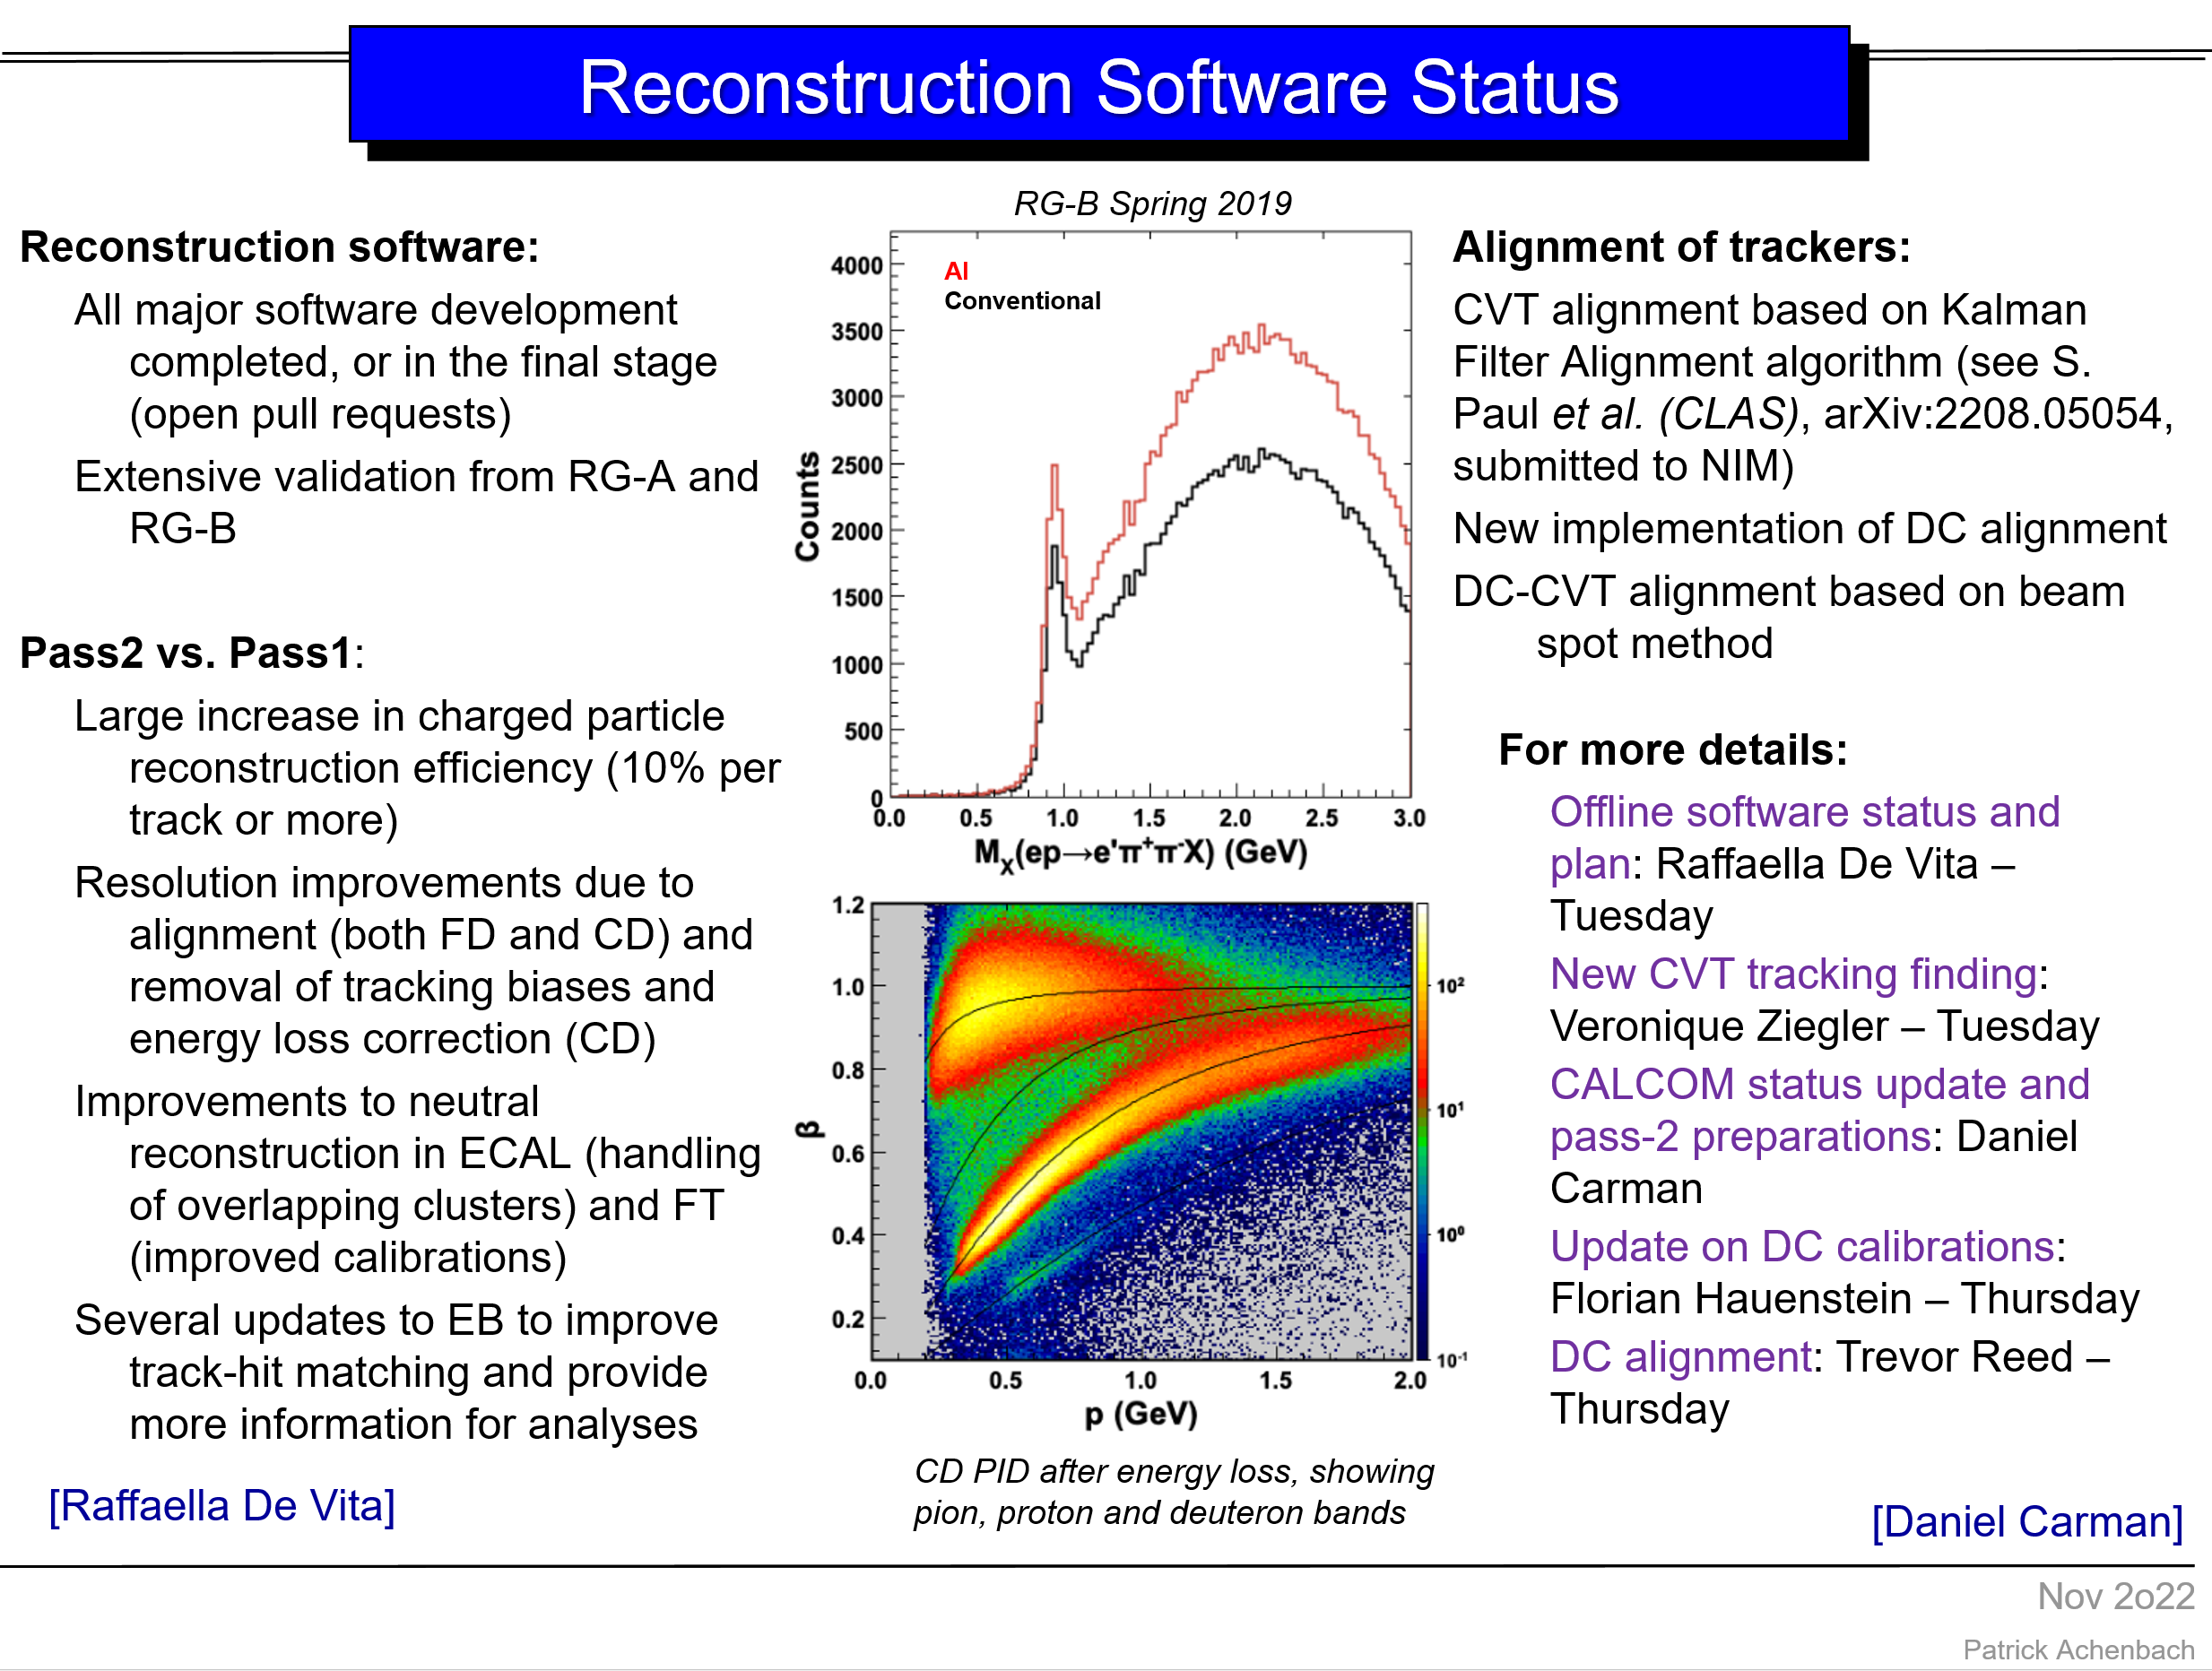
\includegraphics[width=12cm]{Chapters/Ch2-Experiment/recon_pid/pass2vpass1.png}
    			%%%\caption{SVT Strip}
			\end{figure}
			
						
									
			 \begin{figure}[H]
    			\centering
    			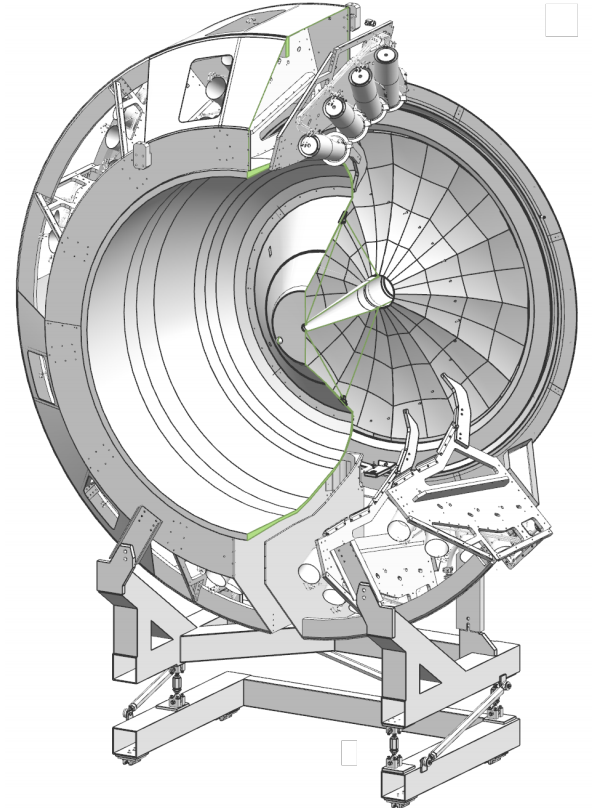
\includegraphics[width=12cm]{Chapters/Ch2-Experiment/clas-12-exp/clas-detectors/fd/pics/htcc.png}
    			%%%\caption{SVT Strip}
			\end{figure}
			
			

        
        \subsubsection{Torus}
        Outbending allows for lower Q2 measurements, inbending allows for slighly higher Q2 measurements. 

            6 coil torus, 4k amps, 3.5 Tesla torodial field, supercritical LHe cooled. 14.2 Megajoules stored energy. 2 Henries of inductance. Field strongest at small angles, weakest at large angles. 
              Inbending vs out bending:
        I have been wondering about this as well. All I know is that inbending and outbending have different acceptances.
        So, I guess some channels prefers inbending while the others do outbending? I’m not sure though. FX claims outbending results have better quality for these days. 
            									
			 \begin{figure}[H]
    			\centering
    			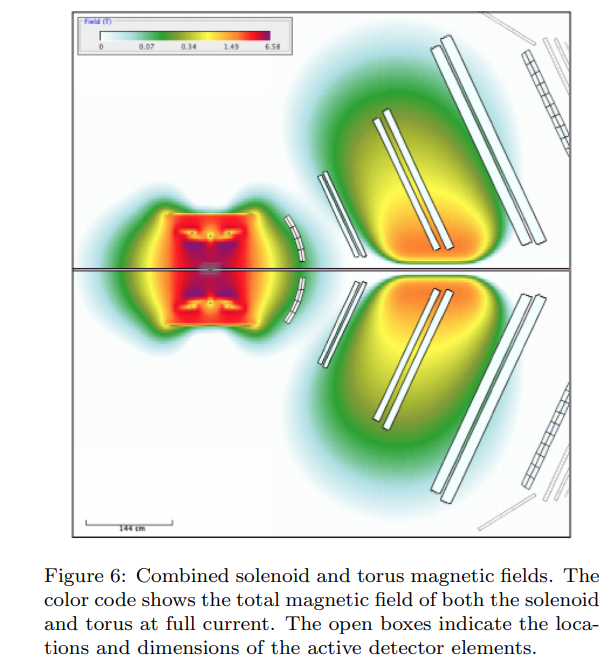
\includegraphics[width=12cm]{Chapters/Ch2-Experiment/clas-12-exp/clas-detectors/fd/pics/torus.png}
    			%%%\caption{SVT Strip}
			\end{figure}
                        

        
        \subsubsection{Drift Chambers}
            There are 3 layers of drift chambers, each with 6 sections. Each chamber has 2 superlayers of 6 layers by 112 wires, for a total of 24,192 wires. (Structure is 112 wires * 6 layers * 2 superlayers * 18 DC sections = 24,192 wires). Physical wire sectioning looks like:\\
            (IIIIII)-(IIIIII)---(IIIIII)-(IIIIII)---(IIIIII)-(IIIIII) x 6 sectors\\
            Where each "I" is a layer of 112 wires.\\
            Spatial resolution is 300 $\mu$ m, angular coverage 5-40 degrees. Momentum resolution $\Delta$p/p < 1\%, angular resolution is 1 mrad in theta, 1mrad/$\sin{\theta}$ for phi. The Drift Chambers are located 2, 3, and 4 meters from the gas mixture is 90/10 Argon/CO2. Time resolution = ?\\
            DC specifics: 30 micron diameter tungsten sense wires, 80 micron Cu-Be field wires, 140 micron Cu-Be guard wires. 20 g tension on sense, 62 g tension of field, 180 g on guard. Max sag calculated to be on order of 10 microns.
            
            									
			 \begin{figure}[H]
    			\centering
    			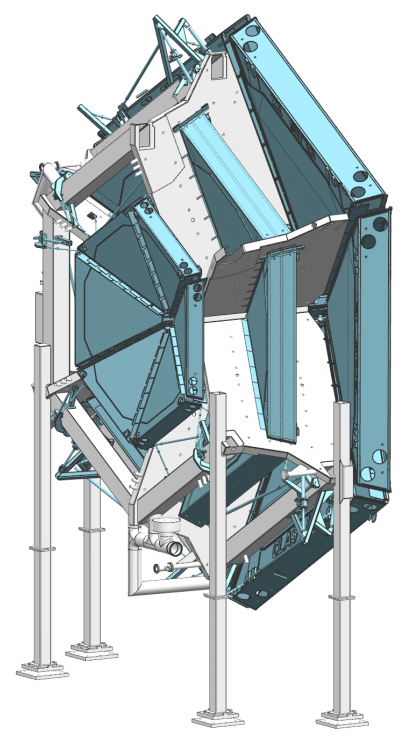
\includegraphics[width=12cm]{Chapters/Ch2-Experiment/clas-12-exp/clas-detectors/fd/pics/drift-chambers.png}
    			%%%\caption{SVT Strip}
			\end{figure}    

            
        \subsubsection{LTCC}
            6 sectors, perfluorobutane ($C_4F_10$) $\longrightarrow$ n = 1.0013 $\longrightarrow$ $\theta_{max}$ = 3 degrees. Electron threshold 9 MeV, pion threshold 2.7 GeV, Kaon threshold 9.4 GeV. Allows for good pion/kaon discrimination from 3.5 Gev to 9 GeV. \\
            Each section has 108 mirrors, 36 winston cones, and 36 PMTs. Mirror is aluminium with $MgF_2$ coating. Kevlar support structure. Perflourobutane is 100\% transparent above 220 nm light. 
            
            
						
									
			 \begin{figure}[H]
    			\centering
    			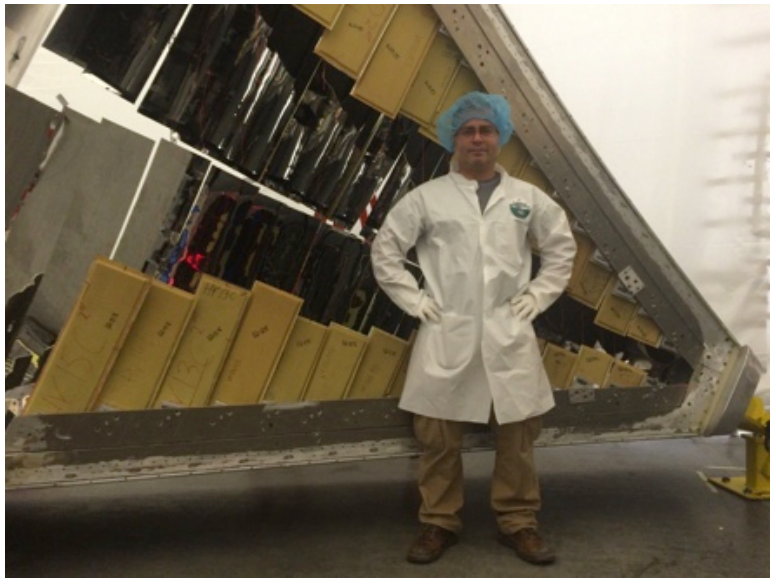
\includegraphics[width=12cm]{Chapters/Ch2-Experiment/clas-12-exp/clas-detectors/fd/pics/ltcc.png}
    			\caption{Low Threshold Chrenkov Counter}
			\end{figure}
			
			

			
        \subsubsection{RICH}
            Provides PID in the range of 3-8 GeV, replacing one sector of LTCC (right middle sector). Pion/Kaon rejection factor > 500, Kaon/Proton rejection factor > 100. Covers 5 to 25 degrees in theta, uses aerogel (n=1.05 $\longrightarrow$ $\theta_{max}$ = 18 degrees). Pion threshold 460 MeV, Kaon threshold 1.6 GeV. Read out by 64 channel photomultipliers. $\beta_{min}$=0.95, $\gamma_{min}$ = 3.3
            
            What is angular resolution?
            
            Reminder of relevant equation:
            \begin{equation}
                \cos{\theta} = \frac{1}{\beta n} \longrightarrow \theta = \arccos{\frac{1}{\beta n}}
            \end{equation}
            
            \begin{equation}
                \gamma = \frac{1}{\sqrt{1-\beta^2}} \longrightarrow \beta = 1-\frac{1}{1-\gamma^2} 
            \end{equation}
            
            \begin{table}[H]
                \centering
                    \begin{tabular}{llll}
                         & momentum & $\sim \gamma$ & $\theta$  \\
                    pion & 3        & 21            & 17.4                      \\
                    kaon & 3        & 6             & 12                        \\
                         &          &               &                         \\
                    pion & 5      & 36            & 17.6                      \\
                    kaon & 5       & 10.1             & 15.9                        \\
                         &          &               &                          \\
                    pion & 8      & 57.1            & 17.7                      \\
                    kaon & 8       & 16             & 17.1                        \\
                    
                    \end{tabular}
            \end{table}
            
        
            
            
            
            \begin{table}[H]
                \centering
                    \begin{tabular}{lll}
                        Detector    &   Scintillator                         &   PMT   \\
                        FTOF - 1a   &     \textcolor{blue}{BC-408}           &   \textcolor{red}{Phillips XP2262, EMI 9954A}\\
                        FTOF - 1b   &     \textcolor{red}{BC-404}           &   \textcolor{blue}{Hama. R9779} \\
                        FTOF - 2    &     \textcolor{blue}{BC-408}           &   \textcolor{magenta}{EMI 4312KB} \\
                        PCAL        &     FNAL                               &   \textcolor{red}{Hama. R6095}\\
                        ECAL        &     \textcolor{cyan}{BC-412}           &   \textcolor{red}{Philips XP2262, EMI 9954}\\
                        CND         &     \textcolor{red}{EJ-200}            &   \textcolor{cyan}{Hama. R10533} \\
                        CTOF        &     \textcolor{blue}{BC-408}           &   \textcolor{green}{Hama. R2083} \\
                        HTCC        &         N/A                            &   ET 9823QKB \\
                        LTCC        &           N/A                          &   200 Photonis XP 4500B\\
                        LTCC        &              N/A                       &   16 Photonis XP 4508 (Quartz Window)\\
                    \end{tabular}
            \end{table}
            
            *ET stands for Electron Tube, a company. Could not find a spec sheet for this PMT type. 
            ** Could not find spec sheets for either HTCC, or LTCC PMTs. 
       
               
            \begin{table}[H]
                \centering
                    \begin{tabular}{lllllll}
                        Scintillator                    & Detectors             &   Principal Use/Features      &   L.O. & WME & R/D Time & L.A. Length \\
                         \textcolor{red}{BC-404}       &  FTOF-1b              &   Fast Counting                   &           68    &   408    & 0.7/1.8           &   140   \\
                         \textcolor{blue}{BC-408}       &  FTOF-1b,2,CTOF       &   TOF - Large Area                &           64    &   425   &   0.9/2.1         &   210  \\
                        \textcolor{cyan}{BC-412}        &  ECAL                 &   Large Area                      &           60   &   434 &   1.0/3/3         &   210\\
                        \textcolor{red}{EJ-200}        &  CND                  &   Long attenuation, fast   &           64     &   425       &   0.9/2.1         &   380   \\
                    \end{tabular}
            \end{table}   
            
            L.O - Light Output - \% Anthracene
            WME - Wavelength Maximum of Emitted Photons
            R/D Time - Rise / Decay time (ns)
            L.A. Length - light attenuation length (cm)
             
             All scintillators have a PVT (Polyvinyltoluene) base. 
             
             EJ-200:          200 -- 10K photons per 1 MeV. 
             
             Thermal effects: EJ-200 loses 5\% of its light output between 20 degrees C and 60 degrees C. No change between -60 to 20 degrees C. 
            
            \begin{table}[H]
                \centering
                %\begin{localsize}{10}
                \scalebox{0.9}{
                    \begin{tabular}{llllllll}
                        PMT                                         & Det.                      &       TS/A    &   WVE         &   PHTC    &   DNY     &       Anode  &    Time Resp.\\ 
                        \textcolor{red}{Hama. R6095}               &  PCAL                     &       28/25   &   300/420/650 & BA/BSG & B\&L/11/2.1  &   1500/0.1    & 4/30/3    \\
                        \textcolor{blue}{Hama. R9779}               &  FTOF-1b                  &       51/46   &   300/420/650 & BA/BSG & LF/8/0.5     &   1750 /0.1   & 1.8/20/0.25 \\
                        \textcolor{cyan}{Hama. R10533}              &  CND                      &       51/46   &   300/420/650 & BA/BSG & LF/10/4.2    &   1000/0.1    &  2/24    \\   
                        \textcolor{green}{Hama. R2083}              &  CTOF                     &       51/46   &   300/420/650 & BA BSG & LF/8/2.5     &   3000/0.2    & 0.7/16/    \\
                        \textcolor{red}{Phillips XP2262}            &  FT1a ECAL            &    &&&&&\\
                        \textcolor{red}{EMI 9954A}                  &  FT1a ECAL            &    &&&&&\\
                        \textcolor{magenta}{EMI 4312KB}             &  FTOF-2                   &    &&&&&\\
                    \end{tabular}}
                %\end{localsize}
            \end{table} 
            
            No spec sheets could be found for the PMTs used in the TFOT1a, ECAL, or FTOF-2.
            Typical dark currents for all PMTs are 100 nA. 
        
            
            Tube size / photocathode area (diameter in mm)
            Wavelength short / peak / long (nm)
            Photocathode / window material (BA = Bialkali, BSG = Borosilicate Glass)
            Dynode structure / stages / gain  LF = Linear-focused, B\&L = Box and line / / Gain - Gain x 10$^6$
            Anode to Cathode Voltage / Anode Current  - Volts / mA
            Rise / transit time/time spread in ns
            
            
            
            \href{https://www.hamamatsu.com/eu/en/product/type/R10533/index.html}{R10533 PMT}
            \href{https://www.hamamatsu.com/eu/en/product/type/R2083/index.html}{R2083 PMT}
            \href{https://pdf1.alldatasheet.com/datasheet-pdf/view/212324/HAMAMATSU/R9779.html}{R9779 PMT}
            \href{https://www.sphere.bc.ca/test/phototubes2/ham/r6095.pdf}{R6095 PMT}
            
            
            
            
            
            
            
            
            
            \href{https://eljentechnology.com/products/plastic-scintillators/ej-200-ej-204-ej-208-ej-212}{CND Scintillator}
            
            
            \href{https://www.crystals.saint-gobain.com/sites/imdf.crystals.com/files/documents/bc400-404-408-412-416-data-sheet.pdf}{BC Scint Specs from Saint Gobain}
            
            
            \href{https://www.hamamatsu.com/eu/en/product/type/R10533/index.html}{CND PMT}
            
            
            \href{https://www.hamamatsu.com/us/en/product/type/R2083/index.html}{CTOF PMT Spec sheet}
            Bialkali photocathode, 8 dynodes, 2.5*10$^6$ typical gain
            Linear-focused dynode structure
            Window material Borosilicate glass
            peak wavelength 420 nm, range from 300 to 650 nm. Max anode to cathode voltage of 3500 V, made anode current of 0.2 mA. Dark current around 100 nA. 
            
            
        
        \subsubsection{FTOF}
            Used for PID, three layer system - 1a, 1b, and 2. Has a design resolution of 60 ps to 160 ps. Average scintillation rate 250 kHz. Pion/Kaon separation up to 2.8 GeV, Kaon Proton separation up to 4.8 GeV, pion proton separation up to 5.4 GeV. \\
            6 meters away from target.
            Time resolution of 80 ps less than 36 degrees, 150 ps greater than 36 degrees. PMTs are shileded from CLAS12 torus. 6 sectors, plastic scintillator, double sided PMT readout. 3 panesl - 1a - 23 counters, 1b - 62 counters, 2 - 5 counters. \\
            15cm wide x 5 cm deep x 33 cm up to 376 cm long.\\
            20-30 cm up to 15x5 130 ps\\
            350-400 cm 6x6 60 ps\\
            370 to 430 cm, 22x5cm, 150 ps\\
            
            									
			 \begin{figure}[H]
    			\centering
    			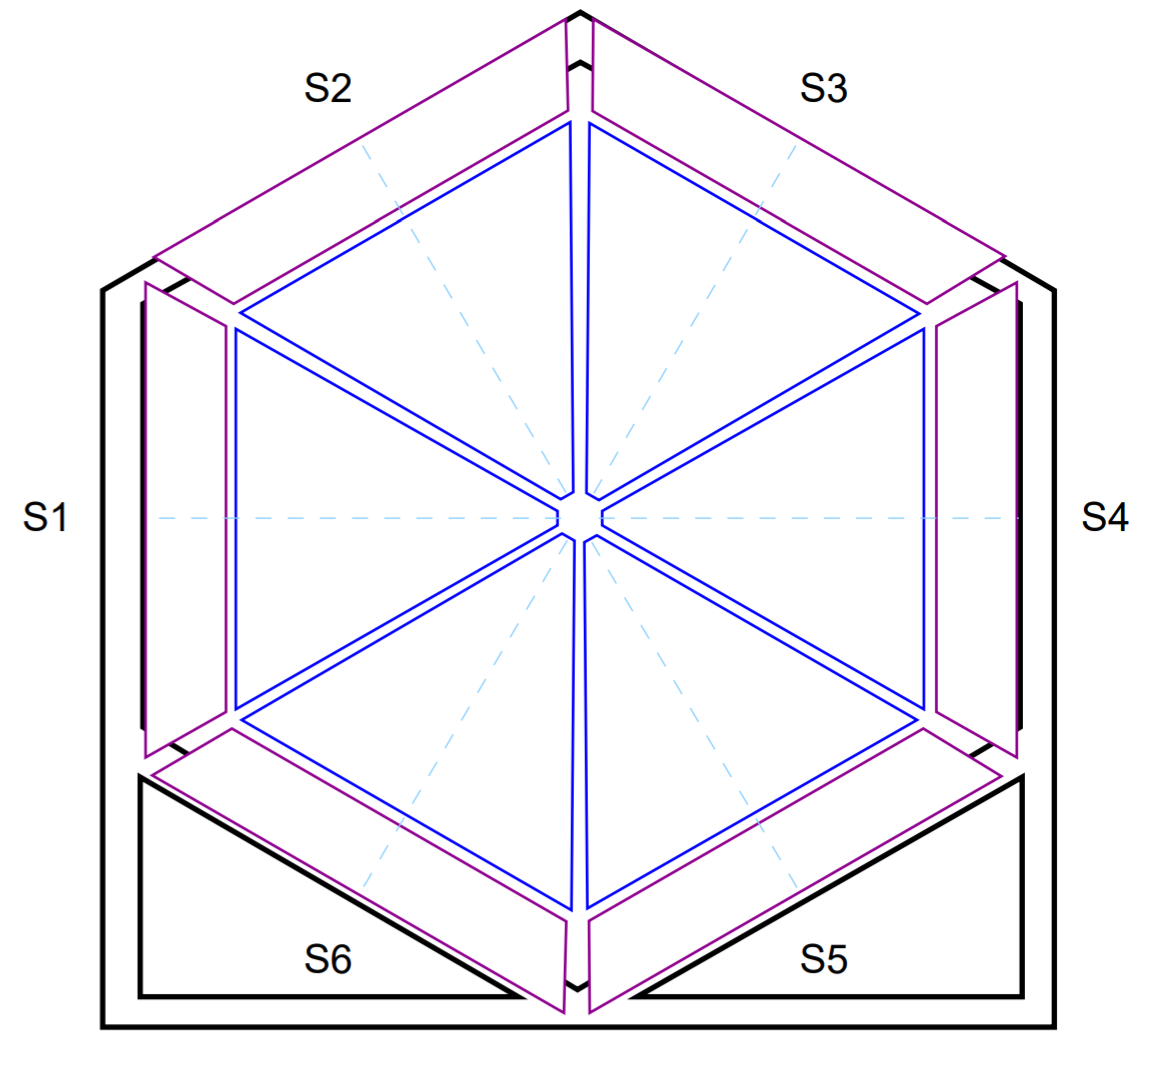
\includegraphics[width=12cm]{Chapters/Ch2-Experiment/clas-12-exp/clas-detectors/fd/pics/ftof-front.png}
    			%%%\caption{SVT Strip}
			\end{figure}

		
			 \begin{figure}[H]
    			\centering
    			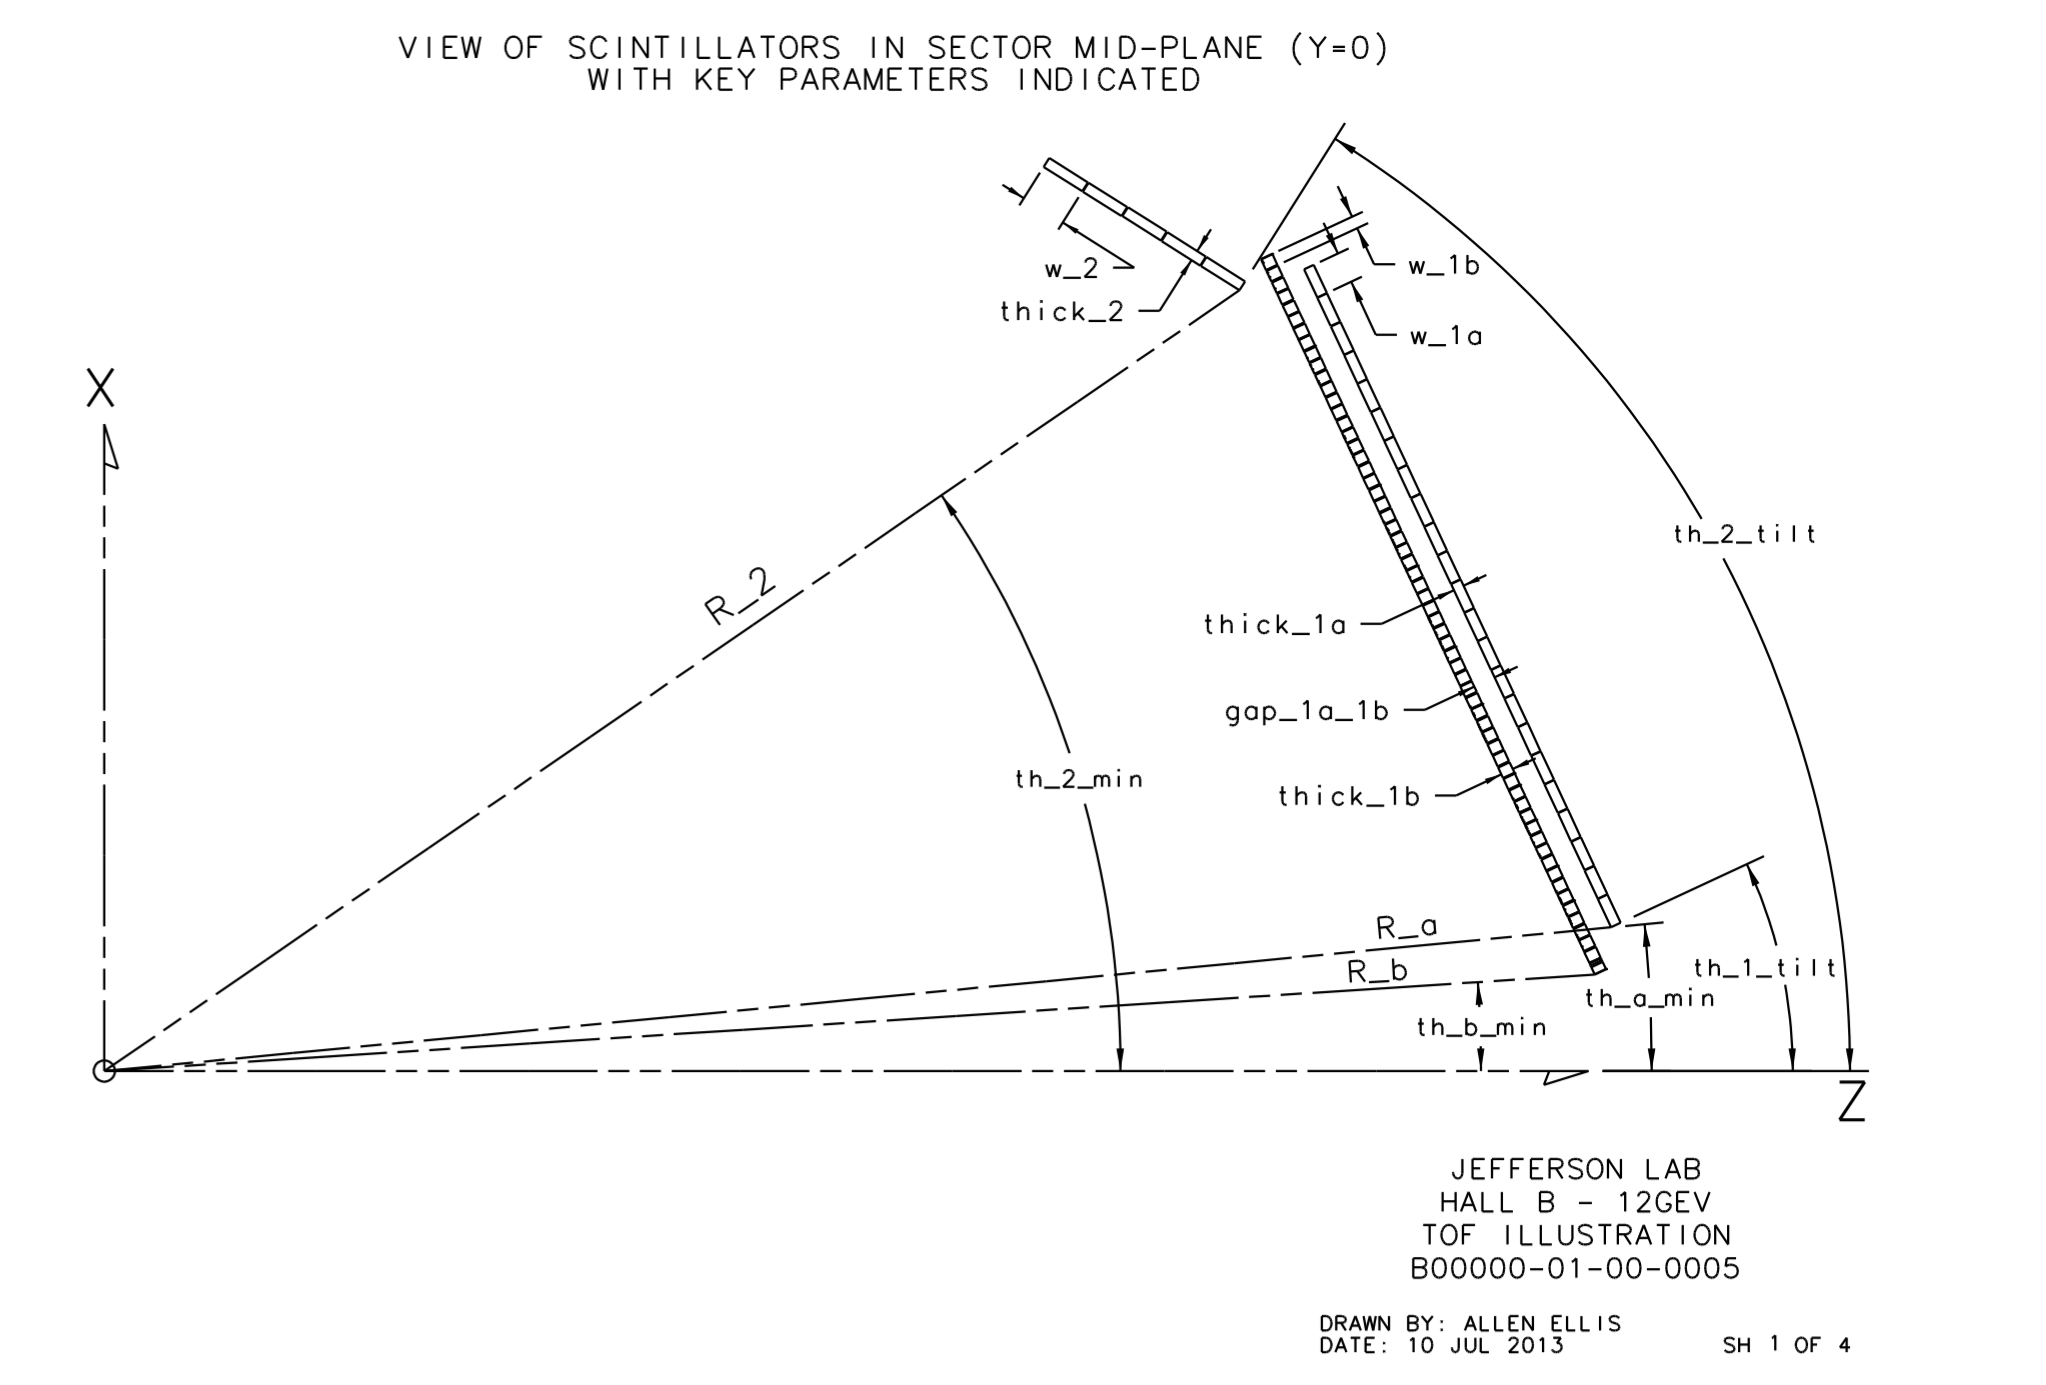
\includegraphics[width=12cm]{Chapters/Ch2-Experiment/clas-12-exp/clas-detectors/fd/pics/clas12-ftof-geom.png}
    			%%%\caption{SVT Strip}
			\end{figure}
			
			
            
            The timing resolution minimums are for being close to the beam axis where particles are moving faster, and farther out from the beamline (larger theta) particles are moving slower so a less resolved time difference is acceptable. 
            
            \paragraph{1a}
                Coverage is 50\% at 5 degrees to 85\% at 35 degrees\\
                Dimensions: L 32.3 cm to 376.1 cm, wxh = 15x5 cm\\
                Material BC-408\\
                PMTS: EMI 9954A, Phillips XP2262\\
                Time resolution 90 - 160 ps small bar to big bars\\
            \paragraph{1b}
                Coverage is 50\% at 5 degrees to 85\% at 35 degrees\\
                Dimensions: L 17.3 cm to 407.9 cm, wxh = 6x6 cm\\
                Material BC-404 (first half) and BC-408\\
                PMTS: Hamamatsu R9779\\
                Time resolution 60-110 ps small bar to big bars\\
            \paragraph{2}
                Coverage is 85\% at 35 degrees to 90\% at 45 degrees\\
                Dimensions: L 371.3 cm to 426.2 cm, wxh = 22x5 cm\\
                Material BC-408\\
                PMTS: EEMI 4312KB\\
                Time resolution 140 - 165 ps small bar to big bars\\
           
           
            For more FTOF specifcications, look \href{https://www.jlab.org/Hall-B/ftof/notes/ftof_geom.pdf}{here} 
                
            FTOF two panels:
Official answer from CLAS12 FTOF NIM paper:
"For tracks that pass through both arrays the combined time information (described in Ref. [10]) is used and results in a 20% improvement compared to using the hit information from panel-1b alone.”, https://www.sciencedirect.com/science/article/pii/S0168900220302102

I guess this is the right answer though:
1a is recycled one from CLAS while 1b is new one.
            
            
        \subsubsection{PCal and ECal}
            ECal from CLAs could only contain showers with E < 5 GeV. Above 5.5 GeV, couldn't resolve neutral pion gamma gamma angle, so needed PCAL. PCAL is 7 meters from target, ECAL is 7.5 M from target. EC segmentation 10 cm, PCAL finer segmentation. PCal 5.5 radiation lengths. 20.5 radiation lengths total. Both are sampling calorimeters, with PB and scintillator layers. The CLAS ECAL was resused and a new PCAL was installed in front of it. Primarily used for identification of electrons, photons, gamma gamma decays from pions, and neutrons. They are sampling calorimeters with six moduels. Each module has a triangular shape with 54 (15/15/24 - PCAL/ECALinner/ECALouter) layers of 1 cm htick scintillators segmented into 4.5/10 cm (PCAL/ECAL) wide strips and sandwiched between 2.2 mm thick lead sheets. The total thickness is about 20.5 radiation lengths. \\
            \indent Scintillator layers are grouped into three readout views with 5/5/8 PCAL/ECinner/ECouter, layers per view providing several cm resolution of energy clusters. Light from each scintillator readout group is routed to PMTs via flexible optical fibers.\\
            Overall perfomance:\\
            Energy resolution of 10\%, position resolution of 2 cm, time resolution of 500 ps. \\
            Are these the real statistics? Because they seem like BS.
            
            
            
            \begin{figure}[H]
    			\centering
    			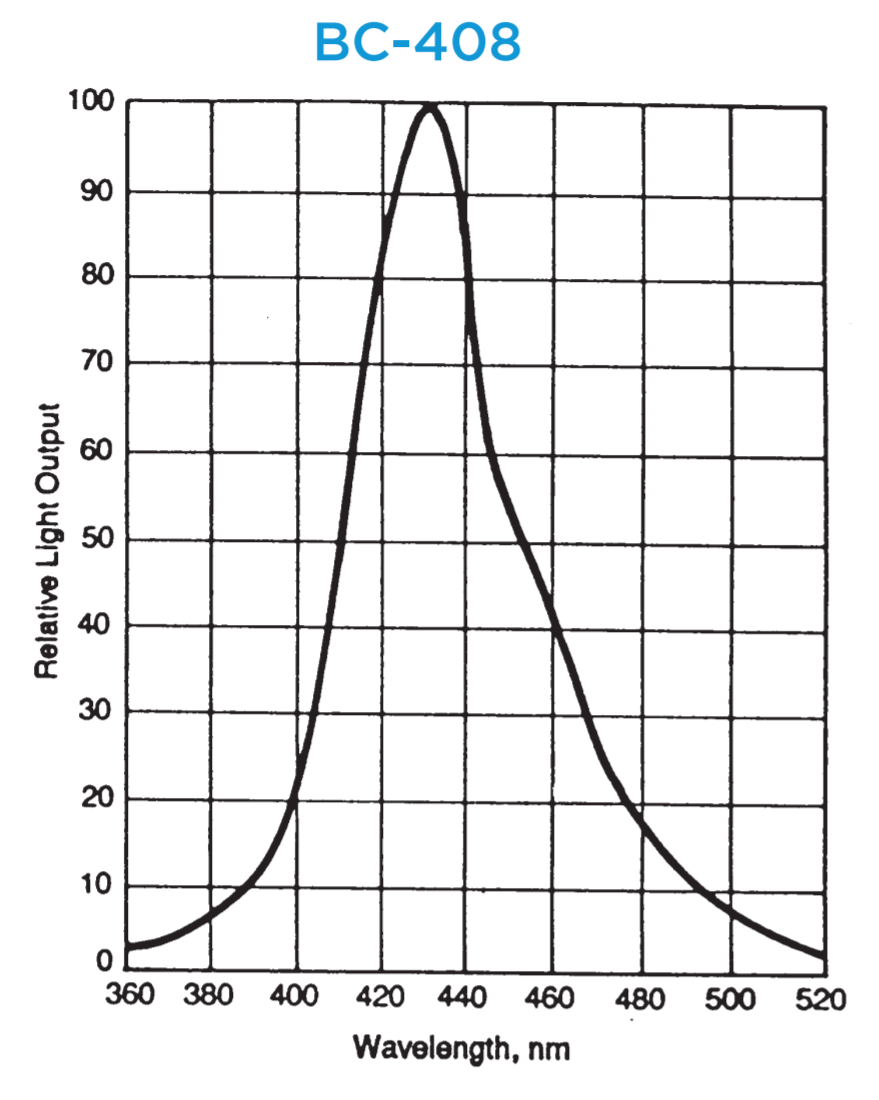
\includegraphics[width=12cm]{Chapters/Ch2-Experiment/clas-12-exp/clas-detectors/fd/pics/sample-BC-408-emission-spectra.png}
    			%\caption{BC 408 Emission Spectra}
			\end{figure}
			
            						
									
			 \begin{figure}[H]
    			\centering
    			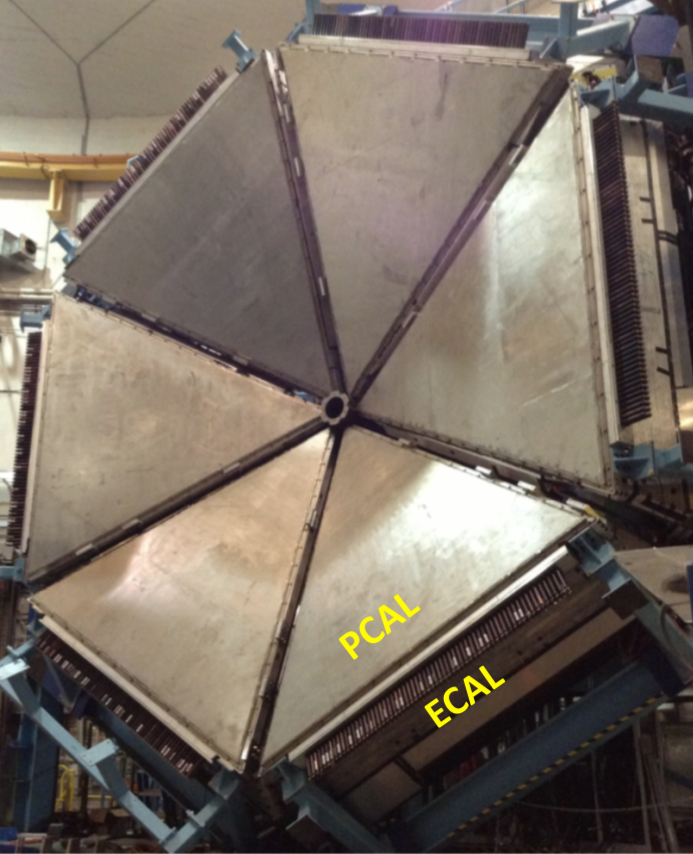
\includegraphics[width=12cm]{Chapters/Ch2-Experiment/clas-12-exp/clas-detectors/fd/pics/clas12-pcal-ecal.png}
    			%%%\caption{SVT Strip}
			\end{figure}
			
			
        \subsubsection{PCAL}
                \indent 50\% coverage at 5 degrees, 85\% coverage at 35 degrees. 15 scintillators, 14 lead layers, per module. 1200 scintillator strips, 1x4.5 cm$^2$ up to 432 cm long, with two holes along the strip, and 0.25 mm TiO2 coating (reflective coating)\\
                Lead sheets are 2.2 mm thick. Readout by fibers into 1 inch PMTs, Hamamatsu R6095. Light yield is 11-12 photo-electrons per MeV. 
                
                PCAL scinitllator was manufactured at the FNAL-NICADD Extrusion Line Facility. Polystyrene base was Dow STYRON 663 W, primary dopant is 2,5 -diphenyloxazole (PPO, 1\% by weight) - this is the organic scintillator, peaks at 385 nm:
                
                
            \begin{figure}[H]
    			\centering
    			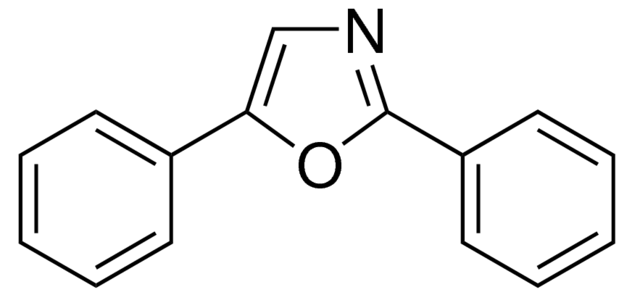
\includegraphics[width=12cm]{Chapters/Ch2-Experiment/clas-12-exp/clas-detectors/fd/pics/2-5-diphenyloxazole.png}
    			%\caption{2,5-diphenyloxazole}
			\end{figure}
                
                The Secondary dopant is 1,4 bis (5-phenyloxazol- 2-yl) benzene (POPOP, 0.03\% by weight) - also scintillator, peaks at 410 nm. 
                
                                
            \begin{figure}[H]
    			\centering
    			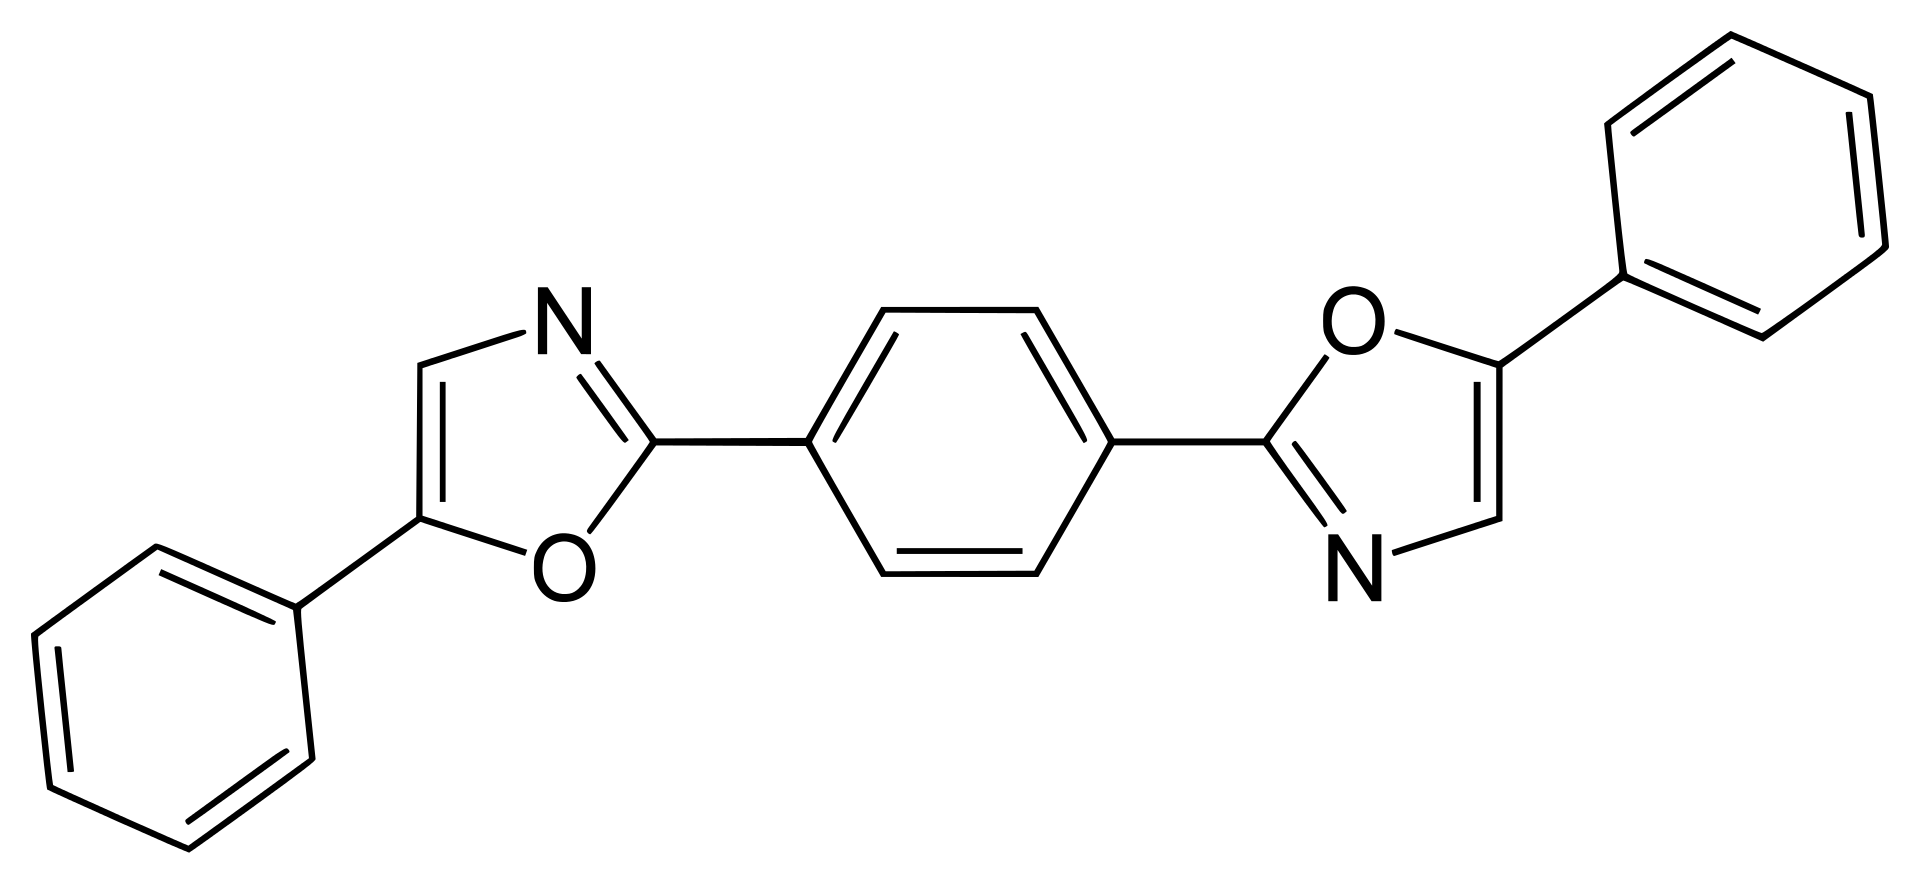
\includegraphics[width=12cm]{Chapters/Ch2-Experiment/clas-12-exp/clas-detectors/fd/pics/popop.png}
    			%\caption{1,4 bis (5-phenyloxazol- 2-yl) benzene}
			\end{figure}
                
                
                
                A reflective surface coating of polystyrene with 12\% TiO2 with 0.25 mm nominal thickness was co-extruded. 
                
                Cast plastic scintillator costs about \$50 per kg, while extruded scintillator is significantly lower in price - about \$10 per kg. 
                
                \href{https://lss.fnal.gov/archive/2005/pub/fermilab-pub-05-344.pdf}{Interesting write up on FNAL Scintillator extrustion}


\href{https://www.sciencedirect.com/science/article/pii/S0168900220300309?via\%3Dihub}{PCal Technical Report}
\href{https://www.sciencedirect.com/science/article/pii/S0168900200009967}{ECal Technical Report}

                
        \subsubsection{ECAL}
                \indent 50\% coverage at 5 degrees, 85\% coverage at 35 degrees. 39/38 scintillators / lead layers per module. 216 readout channels per module, 1200 strips per module. Strips are 1x10to12cm$^2$ by up to 441 cm long, BC-412 (plastic scintillator with high light output, longest light attentuation length, \href{https://www.crystals.saint-gobain.com/products/bc-408-bc-412-bc-416}{cheap!} ). Lead sheets are 2.4 mm thick. Read out by fiber into 2 inch PMTs, Phillips XP2262 and EMI 9954. 3-4 photoelectrons/MeV deposited energy. 


    \subsubsection{Central Detector}
        Overview: The Central Detector spans roughly 35 to 125 degrees, and contains 4 sub-detectors, all in a 5 Tesla solenoidal field. The 5 detectors are: SVT, MMVT, CTOF, and CND. 
        Low t-data are very important for the meson exclusive physics. The GPD interpretation works only in the region -t/Q2<1. From this point of view the central detector will not only increase the total statistics by a factor more than 2 but will add the valuable data with low t.


        \subsubsection{SVT}
            The Silicon Vertex Tracker (SVT) covers from 35 to 125 degrees in $\theta$. Has 8 layers (4 concentric rings) with 10, 14, 18, and 24 sectors respectively, double sided. 2$\pi$ angular coverage. Read out with ASICs- FSSR2s. Designed to operate at $10^{35}$ luminosity, momentum resolution of $\sim$ 5\% for 1 GeV particles with $\theta$ = 90 degrees. 42 cm long, 4 cm wide, 0.4 cm thick. Spatial resolution of 50 $\mu$m, momentum resolution $\sim$ 5\%, theta resolution 10 mrad, phi resolution 5 mrad.  33,792 total readout channels. Sensor thickness is 320 $\mu$m, readout pitch 156 $\mu$ m.Supported by rohacell and carbon fiber backing to reduce material budget, at $\sim 1\%$ of a radiation length.
            
            \begin{figure}[H]
    			\centering
    			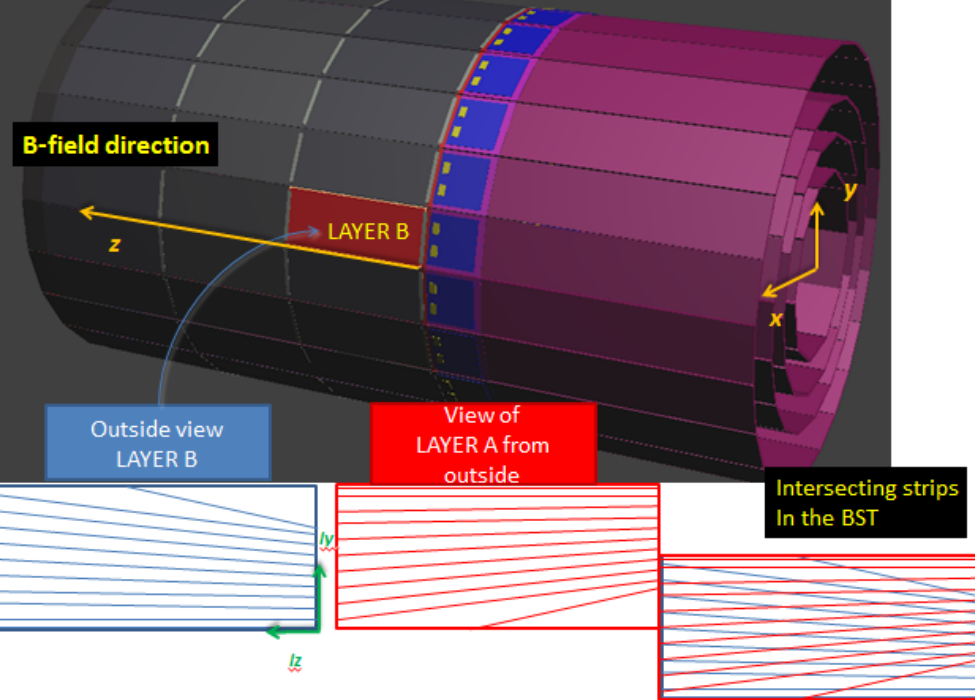
\includegraphics[width=12cm]{Chapters/Ch2-Experiment/clas-12-exp/clas-detectors/cd/pics/svt.png}
    			\caption{Silicon Vertex Tracker}
			\end{figure}  
			
			
			 \begin{figure}[H]
    			\centering
    			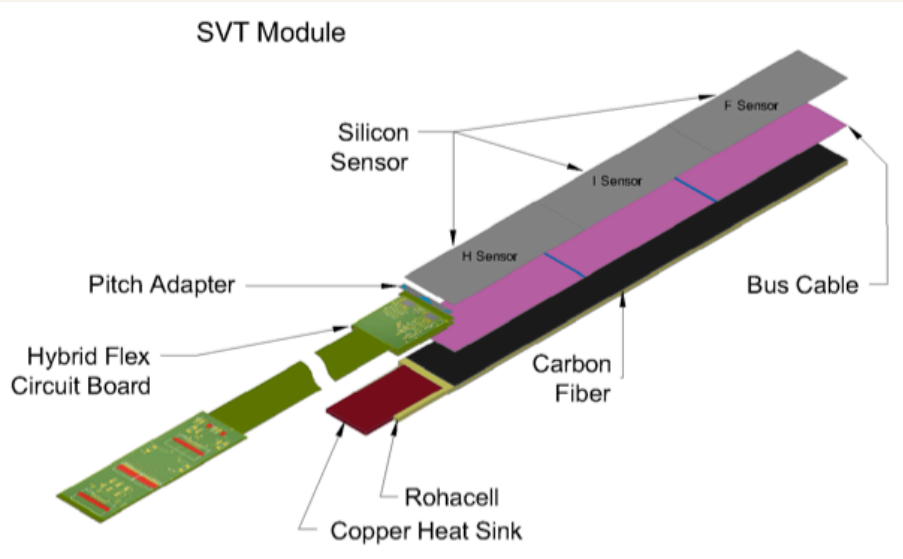
\includegraphics[width=12cm]{Chapters/Ch2-Experiment/clas-12-exp/clas-detectors/cd/pics/svt-module.png}
    			%\caption{SVT Strip}
			\end{figure}  
			
		
		\subsubsection{MMVT}
		    Composed of two parts: a \textbf{Barrel Tracker} and a \textbf{Forward Tracker}. PCB is 200 $\mu$m thick, 0.3\% of a radiation length. 20 MHz sampling frequency. Time resolution of 10 ns. 500 $\mu$m strip pitch.\\
		    \textbf{Advantages of MMVT for CLAS12 :} \\
		    Price: much cheaper compared to SVT. For large area, the price become rapidly prohibitive.
		    Material: Since it is a gasesous detector, it is good for the material budget.
		    Physics Requirements: Not as good spatial resolution as SVT, but can resolve polar angle better. Optimal perform ace is actually achieved with a combination of both detectors are used.
		    \newline
		    Overall momentum uncertainty ($\sigma_p$/p) = 1.6\%. $\sigma_{\theta}$ = 1.4 mrad.  $\sigma_{\phi}$ = 2.6 mrad.  $\sigma _{z}$ = 270 mm.  
		    \subsubsection{Barrel Tracker}
		        18 cylindrical detectors arranged in 6 layers. Covers 35 to 125 degrees. 15,000 readout elements.Gas Mixture 90\% Argon, 10\% isobutane. 3 mm drift gap. 5 kV/cm field. 75\% mesh transparency.
		    \subsubsection{Forward Tracker}
		        6 circular, flat detectors from 6 to 29 degrees in $\theta$. Improves vertex resolution by a factor of up to 10x compared to just the drift chambers along. 6,000 readout elements. 80\% neon, 10\% ethane, 10\% Carbon Tetrafluoride. 5 mm drift gap. 1kV/cm field. 100\% mesh transparency.
		        
		        
		        						
									
			 \begin{figure}[H]
    			\centering
    			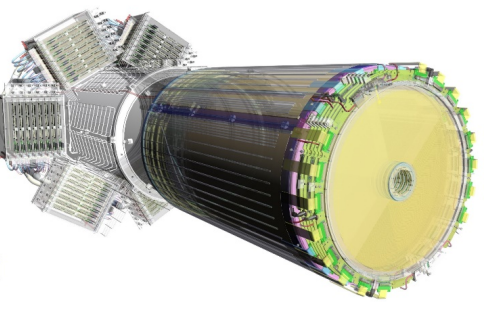
\includegraphics[width=12cm]{Chapters/Ch2-Experiment/clas-12-exp/clas-detectors/cd/pics/MVT.png}
    			%%\caption{SVT Strip}
			\end{figure}
 
    
        \subsubsection{CTOF}
            Central for PID purposes. Divides into 48 1 meter long plastic scintillators with double sided PMT readout.PMTs are in the 0.1 T fringe field region and enclosed in magnetic shielding. 65 picosecond timing resolution. 35 to 125 degrees, 2 $\pi$ in polar angle. 3 cm x 3 cm scintillator planks. Pion/Kaon separation up to 0.64 GeV, Kaon/proton separation up to 1 GeV, pion proton separation up to 1.25 GeV.  
            
            						
			 \begin{figure}[H]
    			\centering
    			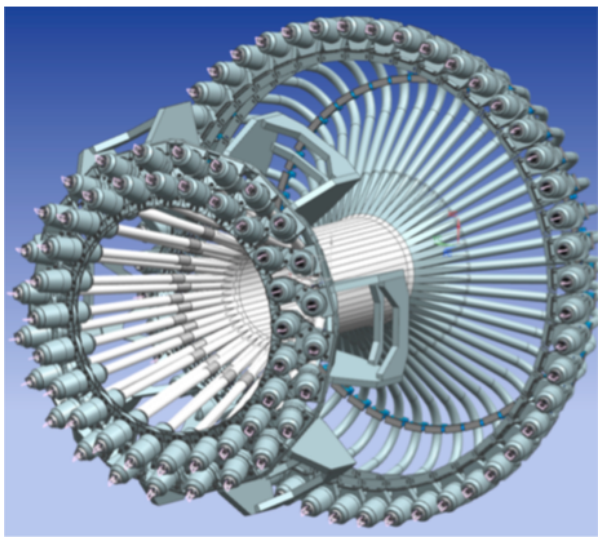
\includegraphics[width=12cm]{Chapters/Ch2-Experiment/clas-12-exp/clas-detectors/cd/pics/CTOF.png}
    			%%\caption{SVT Strip}
			\end{figure}
            
 
		\subsubsection{CND}
		    Detects 0.2-1 GeV neutrons. 3 layers, 48 paddles per layer. Plastic scintillator, 3 cm x 3cm, 0.7 meters  long. Neutron detection efficiency $\sim$ 10\%. 130 picosecond timing resolution, 2 degrees angular resolution (polar and azimuth).
            
            						
			 \begin{figure}[H]
    			\centering
    			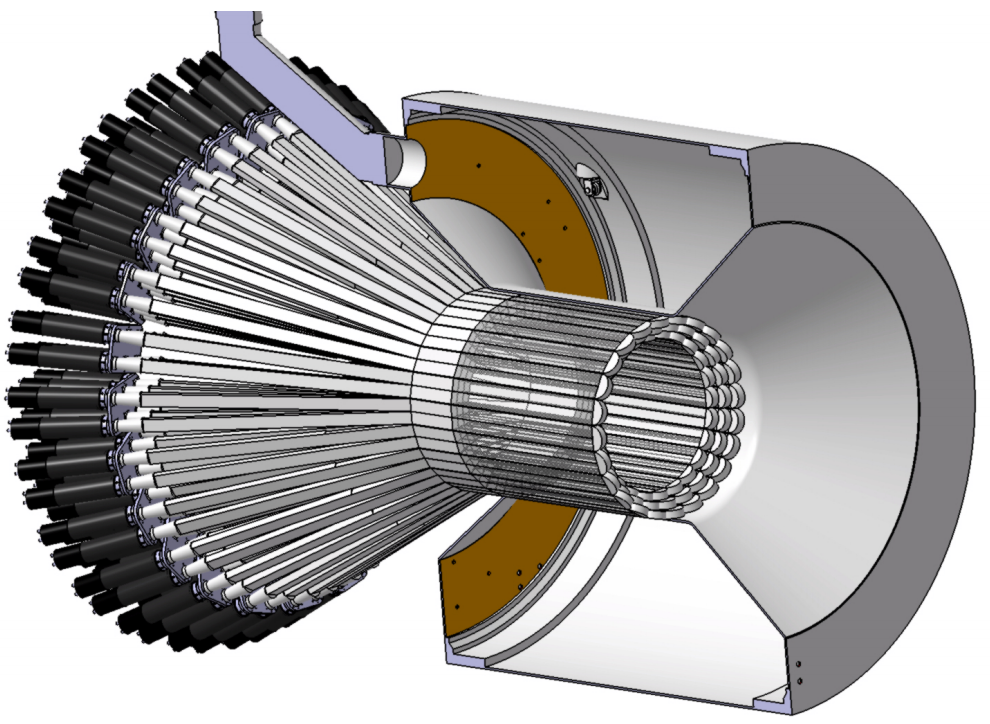
\includegraphics[width=12cm]{Chapters/Ch2-Experiment/clas-12-exp/clas-detectors/cd/pics/CND.png}
    			%%\caption{SVT Strip}
			\end{figure} 

		\subsubsection{Solenoid}
		    5 Tesla super conducting magnet, uniform field ($\Delta$B/B = $10^-4$). Weakest at small angles, strongest at large angles. Opening polar angle of 40 degrees. Momentum range of interest 0.3 to 1.3 GeV. 18 Megajoules stored energy. 85 cm in diameter, 4.2 Kelvin operation. 
		    
    
\subsubsection{Forward Tagger}
    \subsubsection{BAND}
        BAND not impportant.

